%!TEX root = <main.tex>
\section{Incremental Inference Optimizations}\label{sec:exact}
We start with a theoretical characterization of how much speedups we can expect from incremental inference for OBE. We then dive into our novel algebraic framework that enables incremental CNN inference and combine it with our multi-query optimization for OBE.

%inspired by incremental view maintenance in relational databases~\cite{ivm}. We start with a theoretical characterization of how much speedup is possible to set the expectation. We then dive into our novel algebraic framework to enable and optimize incremental inference for OBE. To the best of our knowledge, ours is the first work to combine incremental view maintenance with multi-query optimization for repeated CNN inference.

\vspace{-2mm}
\subsection{Expected Speedups}

\begin{figure}[t]
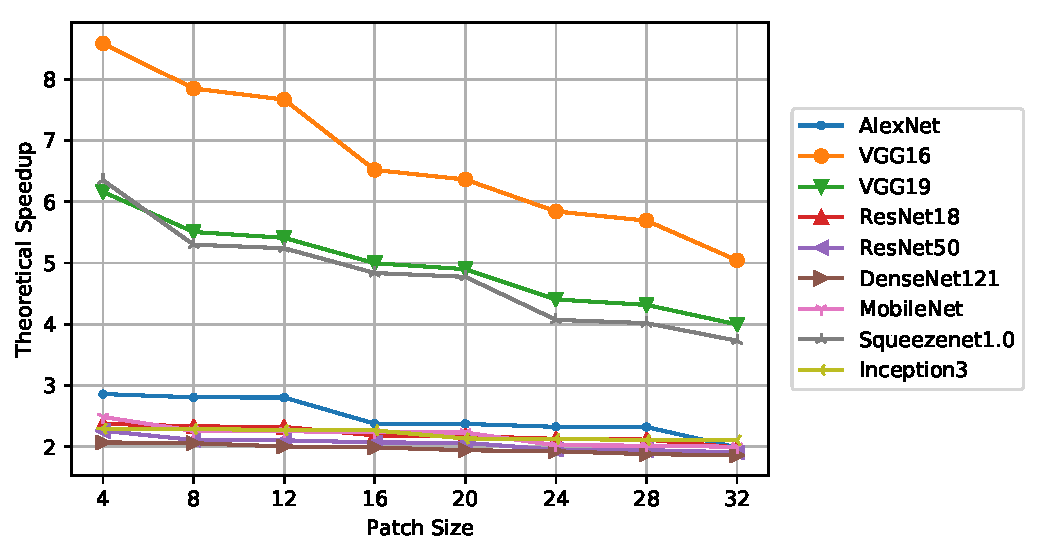
\includegraphics[width=\columnwidth]{images/redundancy_ratio}
\caption{Theoretical speedups for popular deep CNN architectures with incremental inference.}
\label{fig:redundancy_ratio}
\vspace{-8mm}
\end{figure}

The basic reason why IVM offers speedups is that when a part of the input relation is updated, IVM only computes the part of output that gets changed. We bring the IVM notion to CNNs; a CNN layer is our ``query'' and the materialized feature tensor is our ``relation.'' OBE updates only a part of the image; so, only some parts of the tensors need to be recomputed. We create an algebraic framework to determine which parts these are for a CNN layer (Section 3.2) and how to propagate updates across layers (Section 3.3). Given a CNN $f$ and the occlusion patch, our framework determines using ``static analysis'' over $f$ how many FLOPs can be saved. This gives us an upper bound on the possible speedup--we call this the ``theoretical speedup.''
%
More precisely, let the output tensor dimensions of layer $l$ be $(C_{\mathcal{O}:l} , H_{\mathcal{O}:l} , W_{\mathcal{O}:l})$. An incremental update recomputes a smaller local spatial context with width $W_{\mathcal{P}:l} \le W_{\mathcal{O}:l}$ and height $H_{\mathcal{P}:l} \le H_{\mathcal{O}:l}$. Thus, the computational cost of incremental inference for layer $l$, $Q_{inc:l}$, and the total computational cost for incremental inference for $f$, $Q_{inc}$, are given by Equations~(\ref{eqn:inc_local}) and ~(\ref{eqn:inc_all}).

\vspace{-2mm}
\begin{align}
\label{eqn:inc_local}
Q_{inc:l} =&~ (C_{\mathcal{I}:l} \cdot H_{\mathcal{K}:l} \cdot W_{\mathcal{K}:l})  (C_{\mathcal{O}:l} \cdot H_{\mathcal{P}:l} \cdot W_{\mathcal{P}:l})\\
\label{eqn:inc_all}
Q_{inc} =&~ \sum_{l~\mathit{in}~f} Q_{inc:l}
\end{align}

The above costs can be much smaller than $Q_{:l}$ and $Q$ in Equations~(\ref{eqn:full_local}) and~(\ref{eqn:full_all}) earlier.
The \textit{theoretical speedup} is defined as the ratio $\frac{Q}{Q_{inc}}$. It tells us how beneficial incremental inference can be in the best case \textit{without} performing the inference itself. It depends on several factors: the occlusion patch size, its location, the parameters of layers (kernel dimensions, stride, etc.), and so on. Calculating it is non-trivial and requires careful analysis, which we perform. The location of patch affects this ratio because a patch placed in the corner leads to fewer updates overall than one placed in the center of the image. Thus, the ``worst-case'' theoretical speedup is determined by placing the patch at the center.

We performed a sanity check experiment to ascertain the theoretical speedups for a few popular deep CNNs. For varying occlusion patch sizes\eat{worst case: does not matter (with the same stride of 1)}, we plot the theoretical speedups of different deep CNNs. Figure~\ref{fig:redundancy_ratio} shows the results. VGG-16 has the highest theoretical speedups, while DenseNet-121 has the lowest. Most CNNs fall in the 2X--3X range. The differences arise due to the specifics of the CNNs' architectures: VGG-16 has small Convolution filter kernels and strides, which means full inference incurs a high computational cost ($Q = 15$ GFLOPs). In turn, incremental inference is most beneficial for VGG-16. Note that we assumed an image size of $224 \times 224$ for this plot; if the image is larger, the theoretical speedups will be higher.

While one might be tempted to think that speedups of 2X-3X may not be ``that significant'' in practice, we find that they indeed are significant for at least two reasons. First, \textit{users often wait in the loop} for OBE workloads for performing interactive diagnoses and analyses. Thus, even such speedups can improve their productivity, e.g., reducing the time taken on a CPU from about 6min to just 2min, or on a GPU from 1min to just 20s. Second, and equally importantly, incremental inference is the \textit{foundation for our approximate inference} optimizations (Section 4), which amplify the speedups we achieve for OBE. For instance, the speedup for Inception3 goes up from only 2X for incremental inference to up to 8X with all of our optimizations enabled. Thus, incremental inference is critical to optimizing OBE.

\subsection{Single Layer Incremental Inference}\label{sec:inc_computation}

\begin{figure}[t]
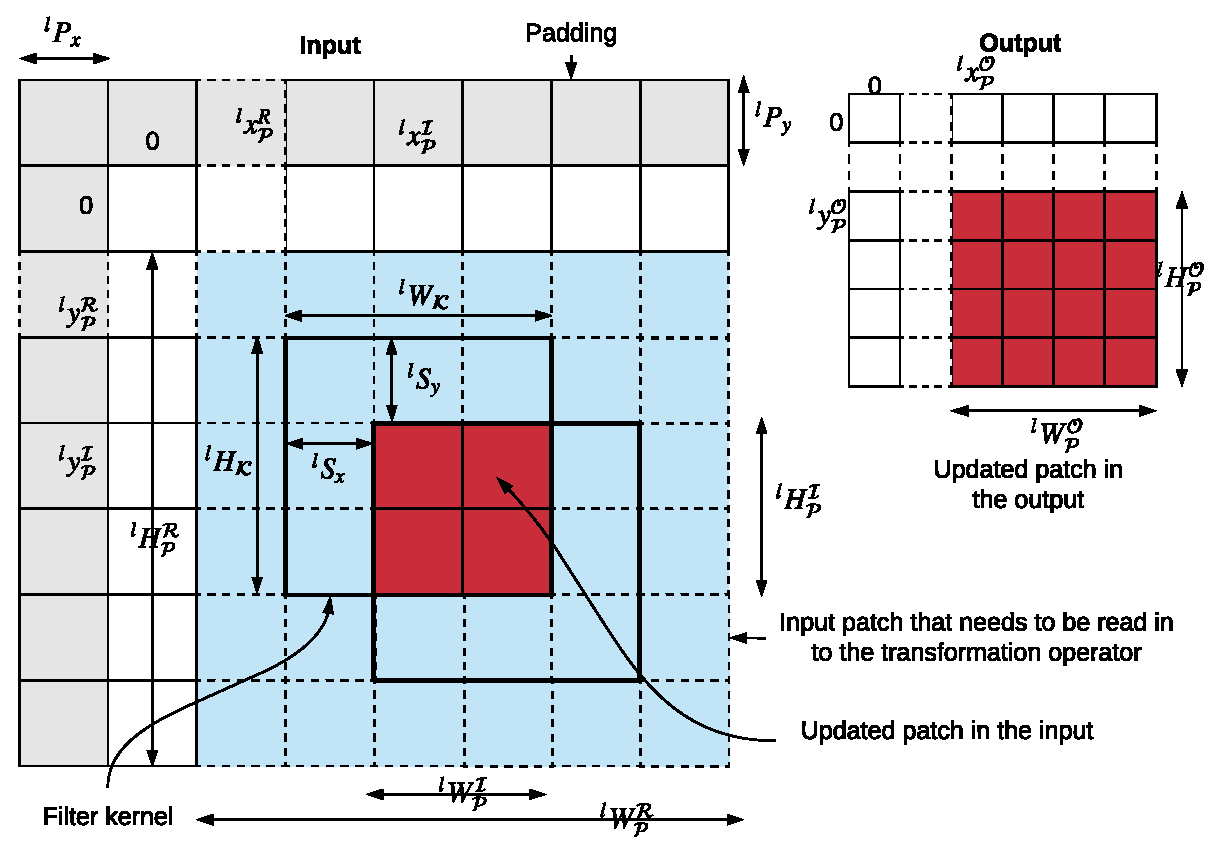
\includegraphics[width=\columnwidth]{images/dimensions}
\vspace{-8mm}
\caption{Simplified illustration of input and output update patches for Convolution/Pooling layers.}
\label{fig:dimensions}
\vspace{-8mm}
\end{figure}

We now present our algebraic framework for incremental updates to the materialized output tensor of a CNN layer. As per the discussion in Section 2.2, we focus only on the non-trivial layers that operate at the granularity of a local spatial context (Convolution and Pooling). We call our modified version of such layers ``incremental inference operations.''

\vspace{2mm}
\noindent \textbf{Determining Patch Update Locations.} We first explain how to calculate the coordinates and dimensions of the \textit{output update patch} of layer $l$ given the \textit{input update patch} and layer-specific parameters. Figure~\ref{fig:dimensions} presents a simplified illustration of these calculations. Our coordinate system's origin is at the top left corner. The input update patch is shown in red/dark color and starts at $(x^\mathcal{I}_{\mathcal{P}:l}, y^\mathcal{I}_{\mathcal{P}:l})$, with height $H^\mathcal{I}_{\mathcal{P}:l}$ and width $W^\mathcal{I}_{\mathcal{P}:l}$. The output update patch starts at $(x^\mathcal{O}_{\mathcal{P}:l}, y^\mathcal{O}_{\mathcal{P}:l})$ and has a height $H^\mathcal{O}_{\mathcal{P}:l}$ and width $W^\mathcal{O}_{\mathcal{P}:l}$. Due to overlaps among filter kernel positions during inference, computing the output update patch requires us to read a slightly larger spatial context than the input update patch--we call this the ``read-in context,'' and it is illustrated by the blue/shaded region in Figure~\ref{fig:dimensions}. The read-in context starts at $(x^\mathcal{R}_{\mathcal{P}:l}, y^\mathcal{R}_{\mathcal{P}:l})$, with its dimensions denoted by $W^\mathcal{R}_{\mathcal{P}:l}$ and $H^\mathcal{R}_{\mathcal{P}:l}$. Table~\ref{table:optimizer_symbols} summarizes all this additional notation for this section. The relationship between these quantities along the width dimension (similarly along the height dimension) can be expressed as follows:

\vspace{-3mm}
\begin{align}
\label{eqn:xcoordinate}
x^\mathcal{O}_{\mathcal{P}:l} =&~ max\big(\lceil (P_{x:l} + x^\mathcal{I}_{\mathcal{P}:l} - W_{\mathcal{K}:l} + 1)/S_{x:l} \rceil, 0\big)\\
\label{eqn:patchwidth}
W^\mathcal{O}_{\mathcal{P}:l} =&~ min\big(\lceil (W^\mathcal{I}_{\mathcal{P}:l} + W_{\mathcal{K}:l} - 1)/ S_{x:l} \rceil, W_{\mathcal{O}:l}\big)\\
\label{eqn:xreadcoordinate}
x^\mathcal{R}_{\mathcal{P}:l} =&~ x^\mathcal{O}_{\mathcal{P}:l} \times S_{x:l} - P_{x:l}\\
\label{eqn:readpatchwidth}
W^\mathcal{R}_{\mathcal{P}:l} =&~ W_{\mathcal{K}:l} + (W^\mathcal{O}_{\mathcal{P}:l}-1) \times S_{x:l}
\end{align}
\vspace{-8mm}

% \begin{align}
% \label{eqn:xcoordinate}
% x^\mathcal{O}_\mathcal{P} =&~ max\big(\lceil (P_x + x^\mathcal{I}_\mathcal{P} - W_\mathcal{K} + 1)/S_x \rceil, 0\big)\\
% \label{eqn:ycoordinate}
% y^\mathcal{O}_\mathcal{P} =&~ max\big(\lceil (P_y + y^\mathcal{I}_\mathcal{P} - H_\mathcal{K} + 1)/S_y \rceil, 0\big)
% \end{align}

% \begin{align}
% \label{eqn:patchwidth}
% W^\mathcal{O}_\mathcal{P} =&~ min\big(\lceil (W^\mathcal{I}_\mathcal{P} + W_\mathcal{K} - 1)/S_x \rceil, W_{\mathcal{O}}\big)\\
% \label{eqn:patchheight}
% H^\mathcal{O}_\mathcal{P} =&~ min\big(\lceil (H^\mathcal{I}_\mathcal{P} + H_\mathcal{K} - 1)/S_y \rceil, H_{\mathcal{O}}\big)
% \end{align}

% \begin{align}
% \label{eqn:xreadcoordinate}
% x^\mathcal{R}_\mathcal{P} =&~ x^\mathcal{O}_\mathcal{P} \times S_x - P_x\\
% \label{eqn:yreadcoordinate}
% y^\mathcal{R}_\mathcal{P} =&~ y^\mathcal{O}_\mathcal{P} \times S_y - P_y
% \end{align}

% \begin{align}
% \label{eqn:readpatchwidth}
% W^\mathcal{R}_\mathcal{P} =&~ W_\mathcal{K} + (W^\mathcal{O}_\mathcal{P}-1) \times S_x\\
% \label{eqn:readpatchheight}
% H^\mathcal{R}_\mathcal{P} =&~ H_\mathcal{K} + (H^\mathcal{O}_\mathcal{P}-1) \times S_y
% \end{align}


Equation~(\ref{eqn:xcoordinate}) calculates the coordinates of the output update patch. Padding effectively shifts the coordinate system and thus, $P_{x:l}$ is added to correct it. Due to overlaps among the filter kernels, the affected region of the input update patch will be increased by $W_{\mathcal{K}:l}-1$, which needs to be subtracted from the input coordinate $x^\mathcal{I}_{\mathcal{P}:l}$. A filter of size $W_{\mathcal{K}:l}$ that is placed starting at $x^\mathcal{I}_{\mathcal{P}:l} - W_{\mathcal{K}:l} + 1$ will see an update starting from $x^\mathcal{I}_{\mathcal{P}:l}$. Equation~(\ref{eqn:patchwidth}) calculates the width of the output update patch. Given these, a start coordinate and width of the read-in context are given by Equations~(\ref{eqn:xreadcoordinate}) and~(\ref{eqn:readpatchwidth}); similar equations hold for the height dimension (skipped for brevity).


\begin{table}[t]
  \centering
  \scalebox{0.8}{\begin{tabular}{p{2cm}p{7.5cm}}
    \toprule
    \textbf{Symbol} & \textbf{Meaning}\\
    \midrule \midrule
    $x^\mathcal{I}_{\mathcal{P}:l}, y^\mathcal{I}_{\mathcal{P}:l}$ & Start coordinates of input update patch for layer $l$\\
    \midrule
    $x^\mathcal{R}_{\mathcal{P}:l}, y^\mathcal{R}_{\mathcal{P}:l}$ & Start coordinates of read-in context for layer $l$\\
    \midrule
    $x^\mathcal{O}_{\mathcal{P}:l}, y^\mathcal{O}_{\mathcal{P}:l}$ & Start coordinates of output update patch for layer $l$\\
    \midrule
    $H^\mathcal{I}_{\mathcal{P}:l}, W^\mathcal{I}_{\mathcal{P}:l}$ & Height and width of input update patch for layer $l$\\
   	\midrule
   	$H^\mathcal{R}_{\mathcal{P}:l}, W^\mathcal{R}_{\mathcal{P}:l}$ & Height and width of read-in context for layer $l$\\
   	\midrule
   	$H^\mathcal{O}_{\mathcal{P}:l}, W^\mathcal{O}_{\mathcal{P}:l}$ & Height and width of output update patch for layer $l$\\
    \midrule
    $\tau$ & Projective field threshold\\
    \midrule
    $r_{drill-down}$ & Drill-down fraction for adaptive drill-down\\
    \bottomrule
  \end{tabular}}
\caption{Additional notation for Sections~\ref{sec:exact} and~\ref{sec:approx}.}
\label{table:optimizer_symbols}
\vspace{-4mm}
\end{table}

\vspace{2mm}
\noindent \textbf{Incremental Inference Operation.}
For layer $l$, given the transformation function $T_{:l}$, the pre-materialized input tensor $\mathcal{I}_{:l}$, input update patch $\mathcal{P}^\mathcal{O}_{:l}$, and the above calculated coordinates and dimensions of the input, output, and read-in context, the output update patch $\mathcal{P}^\mathcal{O}_{:l}$ is computed as follows:

\vspace{-2mm}
\begin{align}
\label{eqn:readin}
\mathcal{U} =&~ \mathcal{I}_{:l}[:,x^\mathcal{R}_{\mathcal{P}:l}:x^\mathcal{R}_{\mathcal{P}:l}+W^\mathcal{R}_{\mathcal{P}:l}, y^\mathcal{R}_{\mathcal{P}:l}: y^\mathcal{R}_{\mathcal{P}:l}+ H^\mathcal{R}_{\mathcal{P}:l}]\\
\label{eqn:superposition}
\mathcal{U} =&~ \mathcal{U} \bm\circ_{(x^\mathcal{I}_{\mathcal{P}:l}-x^\mathcal{R}_{\mathcal{P}:l}),(y^\mathcal{I}_{\mathcal{P}:l}-y^\mathcal{R}_{\mathcal{P}:l})} \mathcal{P}^{\mathcal{I}}_{:l}\\
\label{eqn:callt}
\mathcal{P}^\mathcal{O}_{:l} =&~ T_{:l}(\mathcal{U})
\end{align}

Equation~(\ref{eqn:readin}) slices the read-in context $\mathcal{U}$ from the pre-materialized input tensor $\mathcal{I}_{:l}$. Equation~(\ref{eqn:superposition}) superimposes the input update patch $\mathcal{P}^\mathcal{I}_{:l}$ on it. This is an in-place update of the array holding the read-in context. Finally, Equation~(\ref{eqn:callt}) computes the output update patch $\mathcal{P}^{\mathcal{O}}_{:l}$ by invoking $T_{:l}$ on $\mathcal{U}$. Thus, we avoid performing inference on all of $\mathcal{I}_{:l}$, thus achieving incremental inference and reducing FLOPs.


\subsection{Propagating Updates across Layers}

\vspace{2mm}
\noindent \textbf{Sequential CNNs.} Unlike relational IVM, CNNs have many layers, often in a sequence. This is analogous to having a sequence of queries that require IVM on their predecessor's updated output. This leads to a new issue: correctly and automatically configuring the update patches across all layers of a CNN. Specifically, output update patch $\mathcal{P}^{\mathcal{O}}_{:l}$ of layer $l$ becomes the input update patch of layer $l+1$. While this seems simple, it requires care at the boundary of a local context transformation and a global context transformation, e.g., going from a Convolution layer (or Pooling layer) to a Fully-Connected layer. In particular, we need to materialize the \textit{full updated output} instead of propagating just the output update patches, since the global context transformation might lose spatial locality for subsequent layers.

\vspace{2mm}
\noindent \textbf{Extension to DAG CNNs.} Some recent deep CNNs have a more general directed acyclic graph (DAG) structure for layers. They have two new kinds of layers that ``merge'' two branches in the DAG: \textit{element-wise addition} and \textit{depth-wise concatenation}. Element-wise addition requires two input tensors with all dimensions being identical. Depth-wise concatenation takes two input tensors with the same height and width dimensions. We now face a new challenge--how to calculate the output update patch when the two input tensors differ on their input update patches locations and sizes? Figure~\ref{fig:la_operators} shows a simplified illustration of this issue. The first input has its update patch starting at coordinates $(x^\mathcal{I}_{\mathcal{P}_1:l},y^\mathcal{I}_{\mathcal{P}_1:l})$ with dimensions $H^\mathcal{I}_{\mathcal{P}_1:l}$ and $W^\mathcal{I}_{\mathcal{P}_1:l}$, while the second input has its update patch starting at coordinates $(x^\mathcal{I}_{\mathcal{P}_2:l},y^\mathcal{I}_{\mathcal{P}_2:l})$ with dimensions $H^\mathcal{I}_{\mathcal{P}_2:l}$ and $W^\mathcal{I}_{\mathcal{P}_2:l}$. This issue can arise with both element-wise addition and depth-wise concatenation. 

\begin{figure}[t]
\vspace{-2mm}
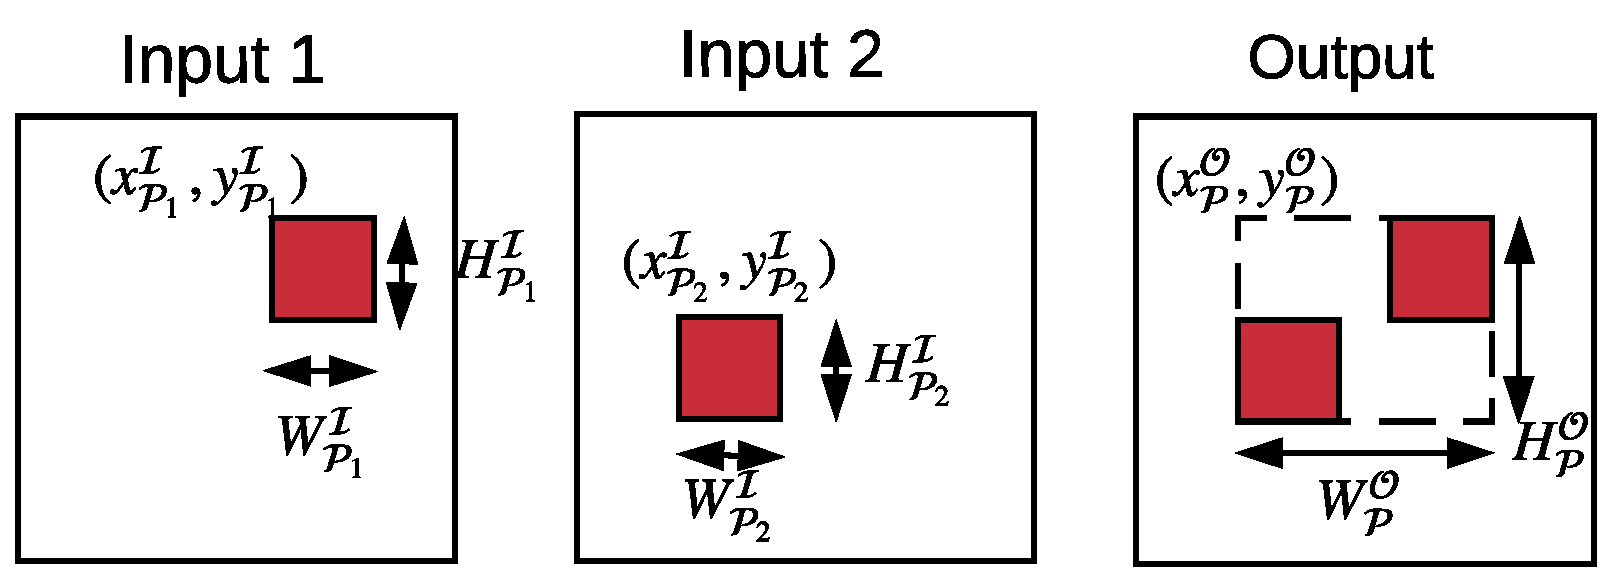
\includegraphics[width=\columnwidth]{images/la_operators}
\caption{Illustration of bounding box calculation for differing input update patch locations for element-wise addition and depth-wise concatenation layers in DAG CNNs.}
\label{fig:la_operators}
\vspace{-4mm}
\end{figure}

We propose a simple unified solution: compute the \textit{bounding box} of the input update patches. So, the coordinates and dimensions of both read-in contexts and the output update patch will be identical. Figure~\ref{fig:la_operators} illustrates this. While this will potentially recompute parts of the output that do not get modified, we think this trade-off is acceptable because the gains are likely to be marginal for the additional complexity introduced into our framework. Overall, the output update patch coordinate and width dimension are given by the following (similarly for the height dimension):

\vspace{-2mm}
\begin{align}
\begin{split}
x^\mathcal{O}_{P:l} =&~ \texttt{min}(x^\mathcal{I}_{\mathcal{P}_1:l}, x^\mathcal{I}_{\mathcal{P}_2:l})\\
% y^\mathcal{O}_\mathcal{P} = y^\mathcal{R}_\mathcal{P} =&~ \texttt{min}(y^\mathcal{I}_{\mathcal{P}_1},y^\mathcal{I}_{\mathcal{P}_2})\\
% \label{eqn:lapatchwidth}
W^\mathcal{O}_{\mathcal{P}:l} =&~ \texttt{max}(x^\mathcal{I}_{\mathcal{P}_1:l}+W^\mathcal{I}_{\mathcal{P}_1:l},x^\mathcal{I}_{\mathcal{P}_2:l}+W^\mathcal{I}_{\mathcal{P}_2:l}) -\texttt{min}(x^\mathcal{I}_{\mathcal{P}_1:l},x^\mathcal{I}_{\mathcal{P}_2:l})
% H^\mathcal{O}_\mathcal{P} = H^\mathcal{R}_\mathcal{P} =&~ \texttt{max}(y^\mathcal{I}_{\mathcal{P}_1}+H^\mathcal{I}_{\mathcal{P}_1},y^\mathcal{I}_{\mathcal{P}_2}+H^\mathcal{I}_{\mathcal{P}_2})-\texttt{min}(y^\mathcal{I}_{\mathcal{P}_1},y^\mathcal{I}_{\mathcal{P}_2})
\end{split}
\end{align}

\subsection{Multi-Query Incremental Inference}
OBE issues $|G|$ re-inference requests \textit{in one go}. Viewing each request as a ``query'' makes the connection with multi-query optimization (MQO)~\cite{sellis1988multiple} clear.
The $|G|$ queries are also \textit{not disjoint}, since the occlusion patch is typically much smaller than the image, which means most the pixels are the same for each query.
Thus, we now extend our IVM framework for one re-inference with an MQO-style optimization fusing multiple re-inference requests.
An analogy with relational queries would be having many incremental update queries on the same relation in one go, with each query receiving a different incremental update. 
%To the best of our knowledge, this is the first known case of combining IVM with MQO, at least for CNN inference.

\vspace{2mm}
\noindent \textbf{Batched Incremental Inference.}
Our optimization works as follows: materialize all tensors \textit{once} and \textit{reuse} them for incremental CNN inference across all $|G|$ queries. Since most of the occluded image pixels are the identical, parts of the tensors will likely be identical too. Thus, we amortize the cost of materializing the tensors across all $|G|$ queries. One might wonder, why not just perform ``batched'' inference for the $|G|$ queries? Batched inference is standard practice today for high-throughput compute hardware like GPUs, since it amortizes CNN set up costs, data movement costs, etc. Batch sizes are picked to optimize hardware utilization. We observed that batching is an \textit{orthogonal} (albeit trivial) optimization compared to our optimization. Thus, we can combine both of these ideas to execute incremental inference in a batched manner. We call this approach ``batched incremental inference.'' Empirically, we found that batching alone yields only limited speedups (under $2$X), but combining batching and incremental inference as we do can amplify the speedups. Algorithm~\ref{alg:incinference} formally presents the batched incremental inference operation for layer $l$.

\begin{algorithm}[t]
    \caption{\textproc{BatchedIncrementalInference}}
    \label{alg:incinference}
    \begin{flushleft}
     \hspace*{1mm} \textbf{Input:} \\
     \hspace*{3mm} $T_{:l}$ : \textit{Original Transformation function}\\
     \hspace*{3mm} $\mathcal{I}_{:l}$ : \textit{Pre-materialized input from original image}\\
     \hspace*{3mm} $[\mathcal{P^I}_{1:l},...,\mathcal{P^I}_{n:l}]$ : \textit{Input patches}\\
     \hspace*{3mm} $[(x^\mathcal{I}_{\mathcal{P}_1:l},y^\mathcal{I}_{\mathcal{P}_1:l}),...,(x^\mathcal{I}_{\mathcal{P}_n:l},y^\mathcal{I}_{\mathcal{P}_n:l})]$ : \textit{Input patch coordinates}\\
     \hspace*{3mm} $W^\mathcal{I}_{\mathcal{P}:l},H^\mathcal{I}_{\mathcal{P}:l}$ : \textit{Input patch dimensions}
    \end{flushleft}

\eat{    \begin{flushleft}
     \hspace*{1mm} \textbf{Output:}\\
     \hspace*{3mm} $[\mathcal{P^O}_{1:l},...,\mathcal{P^O}_{n:l}]$ : \textit{Output patches}\\
     \hspace*{3mm} $[(x^\mathcal{O}_{\mathcal{P}_1:l},y^\mathcal{O}_{\mathcal{P}_1:l}),...,(x^\mathcal{O}_{\mathcal{P}_n:l},y^\mathcal{O}_{\mathcal{P}_n:l})]$ : \textit{Output patch coordinates}\\
     \hspace*{3mm} $W^\mathcal{O}_{\mathcal{P}:l},H^\mathcal{O}_{\mathcal{P}:l}$ : \textit{Output patch dimensions}
    \end{flushleft}}

    \begin{algorithmic}[1]
    \Procedure{BatchedIncrementalInference}{}
    \State \textit{Calculate} $[(x^\mathcal{O}_{\mathcal{P}_1:l},y^\mathcal{O}_{\mathcal{P}_1:l}),...,(x^\mathcal{O}_{\mathcal{P}_n:l},y^\mathcal{O}_{\mathcal{P}_n:l})]$ 
    \State \textit{Calculate} ($W^\mathcal{O}_{\mathcal{P}:1},H^\mathcal{O}_{\mathcal{P}:l}$)
    \State \textit{Calculate} $[(x^\mathcal{R}_{\mathcal{P}_1:l},y^\mathcal{R}_{\mathcal{P}_1:l}),...,(x^\mathcal{R}_{\mathcal{P}_n:l},y^\mathcal{R}_{\mathcal{P}_n}:l)]$
    \State \textit{Calculate} ($W^\mathcal{R}_{\mathcal{P}:l},H^\mathcal{R}_{\mathcal{P}:l}$)
    \State \textit{Initialize} $\mathcal{U} \in \mathcal{\rm I\!R}^{n \times \texttt{depth}(\mathcal{I}_{:l}) \times H^\mathcal{R}_{\mathcal{P}:l} \times W^\mathcal{R}_{\mathcal{P}:l}}$

    \For{\texttt{i in [1,...,n]}}\label{alg:line:memcpy_loop}
        \State $T_1 \gets \mathcal{I}_{:l}[:,x^\mathcal{R}_{\mathcal{P}_i:l}:x^\mathcal{R}_{\mathcal{P}_i:l}+W^\mathcal{R}_{\mathcal{P}:l},y^\mathcal{R}_{\mathcal{P}_i:l}:y^\mathcal{R}_{\mathcal{P}_i:l}+H^\mathcal{R}_{\mathcal{P}:l}]$ 
        \State $T_2 \gets T_1 \bm\circ_{(x^\mathcal{I}_{\mathcal{P}_i:l}-x^\mathcal{R}_{\mathcal{P}_i:l}),(y^\mathcal{I}_{\mathcal{P}_i:l}-y^\mathcal{R}_{\mathcal{P}_i:l})} \mathcal{P}_{i:l}$
        \State $\mathcal{U}[i,:,:] \gets T_2$
    \EndFor

    \State $[\mathcal{P}^\mathcal{O}_{1:l},...,\mathcal{P}^\mathcal{O}_{n:l}] \gets T(\mathcal{U})$ \Comment{Batched version}
    \State \textbf{return} $[\mathcal{P}^\mathcal{O}_{1:l},...,\mathcal{P}^\mathcal{O}_{n:l}]$,
    \State \hspace*{5mm} $[(x^\mathcal{O}_{\mathcal{P}_1:l},y^\mathcal{O}_{\mathcal{P}_1:l}),...,(x^\mathcal{O}_{\mathcal{P}_n:l},y^\mathcal{O}_{\mathcal{P}_n:l})],$ ($W^\mathcal{O}_{\mathcal{P}:l},H^\mathcal{O}_{\mathcal{P}:l}$) 
    \EndProcedure
    \end{algorithmic}

% \eat{%Maybe in the Appendix
%     \vspace*{-2mm}
%     \hrulefill
    
%     \begin{flushleft}
%      \hspace*{4mm} \textbf{Input:}\\
%      \hspace*{8mm} $\mathcal{O}$ : \textit{Pre-materialized output from original image}\\
%      \hspace*{8mm} $[\mathcal{P}^\mathcal{O}_1,...,\mathcal{P}^\mathcal{O}_n]$ : \textit{Output patches}\\
%      \hspace*{8mm} $[(x^\mathcal{O}_{\mathcal{P}_1},y^\mathcal{O}_{\mathcal{P}_1}),...,(x^\mathcal{O}_{\mathcal{P}_n},y^\mathcal{O}_{\mathcal{P}_n})]$ : \textit{Output patch coordinates}\\
%     \end{flushleft}

%     \begin{flushleft}
%      \hspace*{4mm} \textbf{Output:}\\
%      \hspace*{8mm} $O\textrm'$ : \textit{Updated output}
%     \end{flushleft}
%   \begin{algorithmic}[1]
%     \Procedure{IncrementalToFullProjection}{}
%     \State \textit{Initialize} $\mathcal{O}\textrm' \in \mathcal{\rm I\!R}^{n \times \texttt{depth}(\mathcal{O}) \times \texttt{height}(\mathcal{O}) \times \texttt{width}(\mathcal{O})}$
%     \For{\texttt{i in [1,...,n]}}
%       \State $T \gets \texttt{copy}(O)$
%       \State $\mathcal{O}\textrm'[i,:,:] \gets T \bm\circ_{x^\mathcal{O}_{\mathcal{P}_i},y^\mathcal{O}_{\mathcal{P}_i}} \mathcal{P}^\mathcal{O}_i$
%     \EndFor
%     \State \textbf{return} $\mathcal{O}\textrm'$
%     \EndProcedure
%     \end{algorithmic}
% }
\end{algorithm}


\eat{
The \textproc{BatchedIncrementalInference} procedure takes in the original transformation of the layer, pre-materialized input for the layer corresponding to the original image, a batch of updated patches which are 3D volumes of activation values and their geometric properties as input.
}

\textproc{BatchedIncrementalInference} first calculates the geometric properties of the output update patches and read-in contexts. A temporary tensor $\mathcal{U}$ is initialized to hold the input update patches with their read-in contexts. The \textbf{for} loop iteratively populates $\mathcal{U}$ with corresponding patches. Finally, $T_{:l}$ is applied to $\mathcal{U}$ to compute the output patches. We note that only for the first layer, all input update patches will be identical to the occlusion patch. But for the later layers, the update patches will start to deviate depending on their locations and read-in contexts.


\vspace{2mm}
\noindent \textbf{GPU Optimized Implementation.}
Empirically, we found a dichotomy between CPUs and GPUs: \textproc{BatchedIncrementalInference} yielded expected speedups on CPUs, but it performed dramatically poorly on GPUs. In fact, a naive implementation of \textproc{BatchedIncrementalInference} on GPUs was \textit{slower} than full re-inference! We now shed light on why this is the case and how we tackled this issue. The \textbf{for} loop in line~\ref{alg:line:memcpy_loop} of Algorithm~\ref{alg:incinference} is essentially preparing the input for $T_{:l}$ by copying values (slices of the materialized tensor) from one part of GPU memory to another sequentially. A detailed profiling of the GPU showed that these \textit{sequential memory copies are a bottleneck} for GPU throughput, since they throttle it from exploiting its massive parallelism effectively. To overcome this issue, we created a custom CUDA kernel to perform input preparation more efficiently by \textit{copying memory regions in parallel} for all items in the batched inference request. This is akin to a parallel \textbf{for} loop tailored for slicing the tensor. We then invoke $T_{:l}$, which is already hardware-optimized by modern deep learning tools~\cite{chetlur2014cudnn}. We defer more details on our custom CUDA kernel to the appendix due to space constraints. Also, since GPU memory might not be enough to fit all $|G|$ queries, the batch size for GPU execution might be smaller than $|G|$.
%\red{TODO: Refer to hardware works, e.g. Li Tseng, Lin, Swanson, Yannis on hardware accelerators}


\vspace{-2mm}
\subsection{Putting it All Together}

We summarize the end-to-end workflow of our incremental inference optimizations for OBE. We are given the CNN $f$, image $\mathcal{I}_{:img}$, predicted class label $L$, occlusion patch $\mathcal{P}$ and its stride $S_{\mathcal{P}}$, and the set of occlusion patch positions $G$. Pre-materialize the output tensors of all layers of $f$ with $\mathcal{I}_{:img}$ as the input. Prepare occluded images ($\mathcal{I}^{'}_{(x,y):img}$) for all positions in $G$. For batches of $\mathcal{I}^{'}_{(x,y):img}$ as the input, invoke the transformations functions of the layers of $f$ in topological order and calculate the corresponding entries of heat map $M$. 
For transformations with local spatial context, invoke \textproc{BatchedIncrementalInference}. For layer that precede a global context transformation, materialize the full updated output. For all other layers, invoke the original transformation function. $M$ is now the output heat map.


\vspace{-2mm}
\section{Approximate Inference Optimizations}\label{sec:approx}
Since incremental inference is \textit{exact}, i.e., it yields the same heat map as full inference, it does not exploit a capability of human perception: tolerance of some degradation in visual quality. Thus, we now build upon our IVM framework to create two novel heuristic approximate inference optimizations that trade off the heat map's quality in a user-tunable manner to accelerate OBE further. We first explain the techniques and then explain how to tune them.

\subsection{Projective Field Thresholding}

\begin{figure}[t]
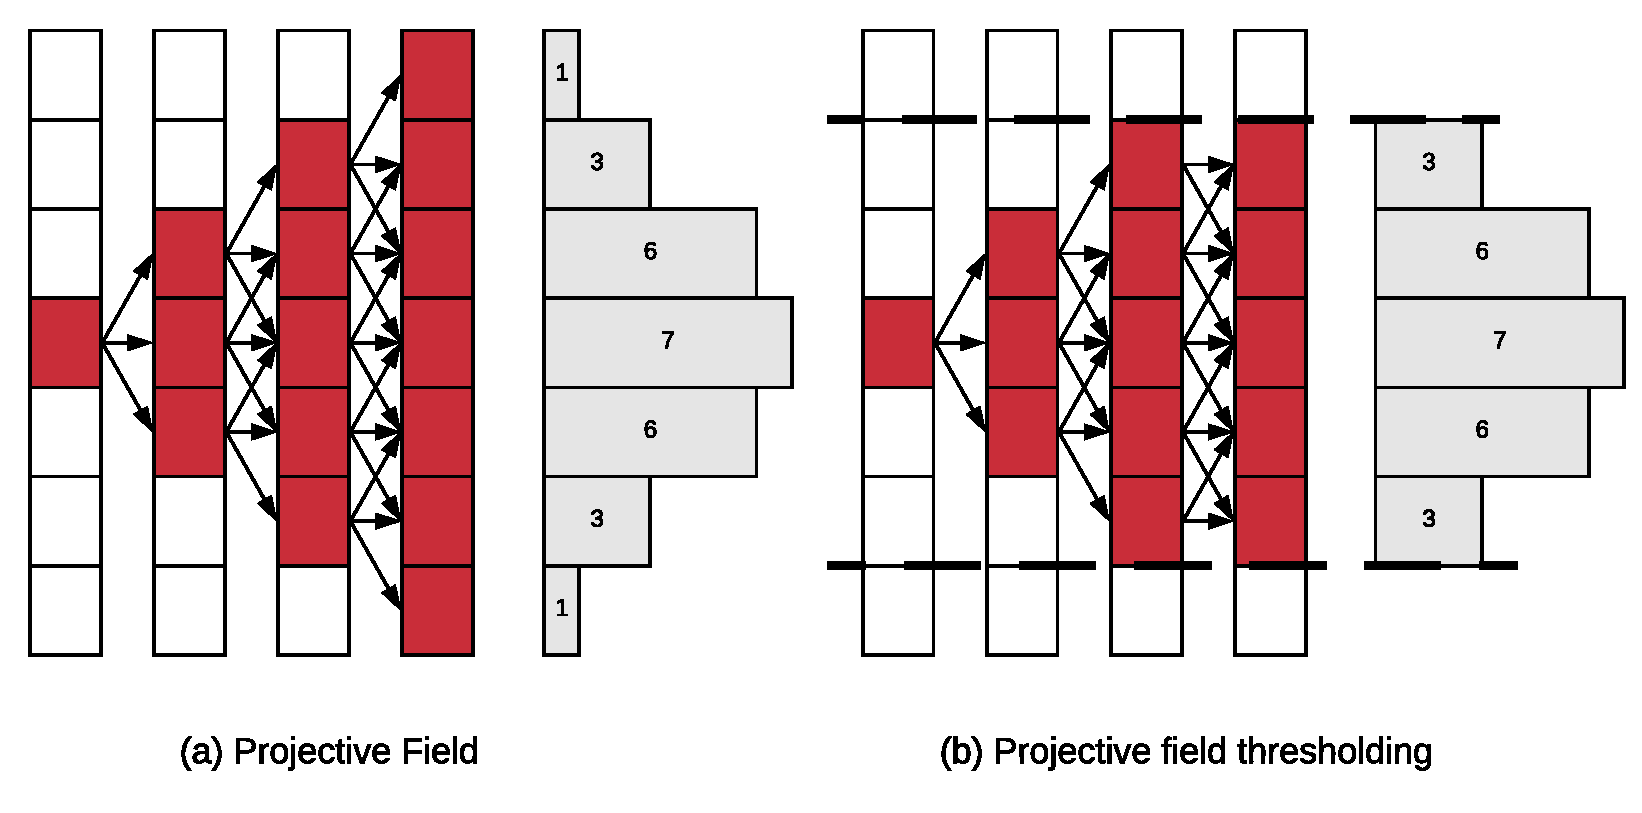
\includegraphics[width=\columnwidth]{images/pf_truncate}
\caption{(a) Projective field growth for 1-D Convolution (filter size $2$, stride $1$). (b) Projective field \textit{thresholding}; $\tau = 5/7$.}
\label{fig:pf_truncate}
\end{figure}

\begin{figure}[t]
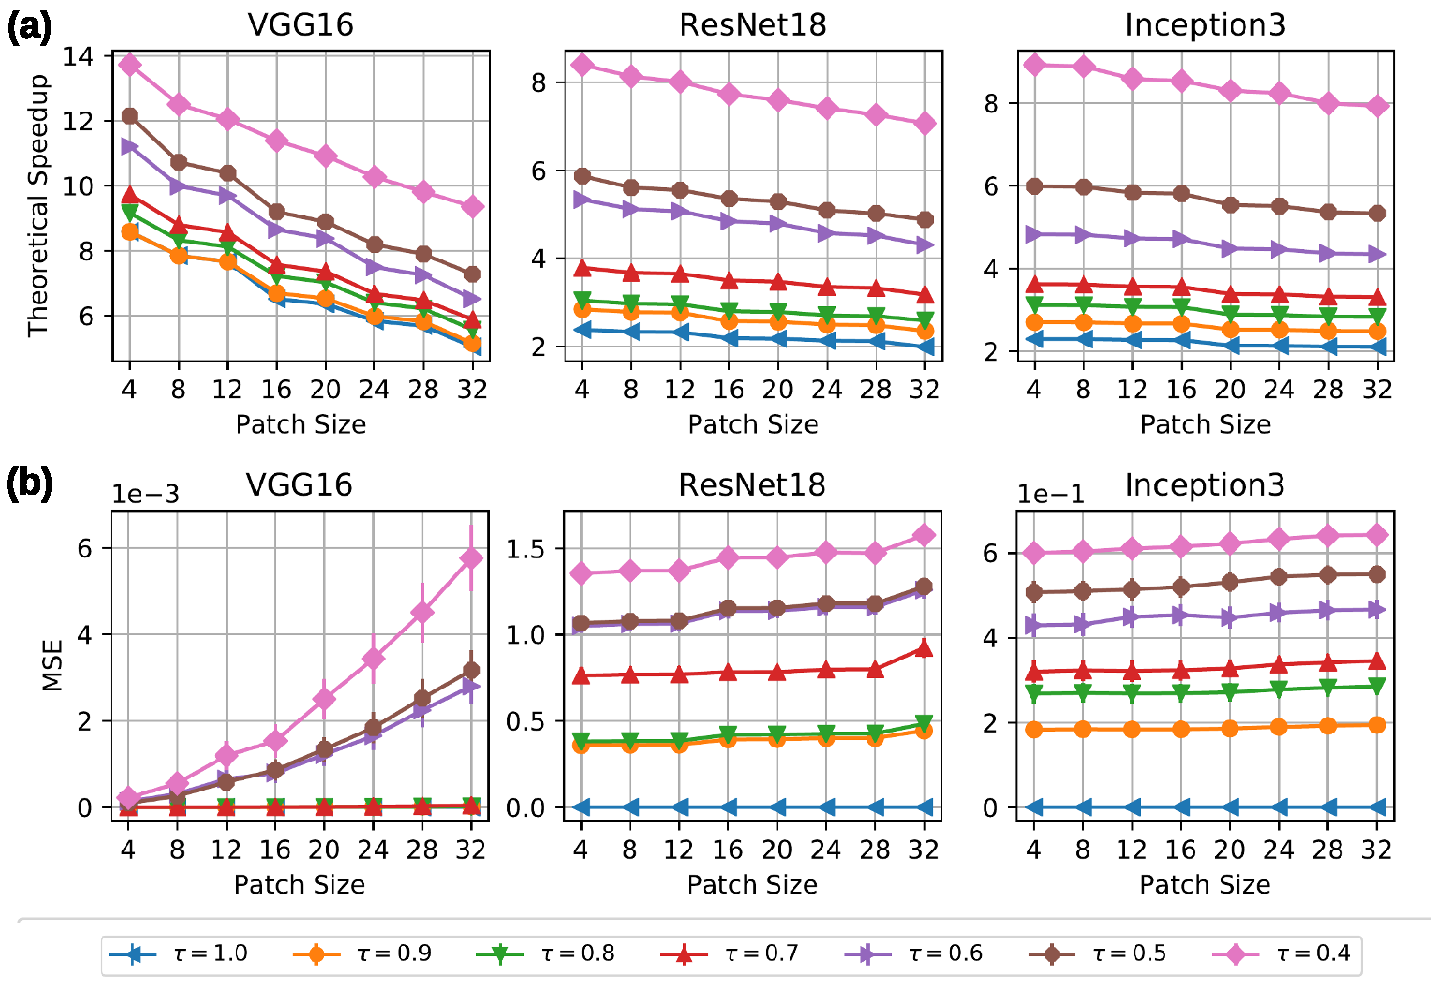
\includegraphics[width=\columnwidth]{images/proj_thresholding}
\caption{(a) Theoretical speedups with projective field thresholding. (b) Mean Square Error between exact and approximate output of final Convolution/Pooling layers.}
\label{fig:proj_thresholding}
\vspace{-4mm}
\end{figure}

The \textit{projective field} of a CNN neuron is the slice of the output tensor that is connected to it~\cite{le2017receptive, basiccnnoperations}. It is a term from neuroscience to describe the effects of a retinal cell on the output of the eye's neuronal circuitry~ \cite{de2011projective}. This notion sheds light on the \textit{growth of the size} of the update patches through the layers of a CNN. The 3 kinds of layers (Section 2.2) affect the projective field size growth differently. Transformations at the granularity of individual elements do not alter the projective field size. Global context transformations increase it to the whole output. But local spatial context transformations, which are the most crucial, increase it \textit{gradually} at a rate determined by the filter kernel's size and stride: additively in the size and multiplicatively in the stride. The growth of the projective field size implies the amount of FLOPs saved by IVM decreases as we go to the higher layers of a CNN. Eventually, the output update patch becomes as large as the output tensor. This growth is illustrated by Figure~\ref{fig:pf_truncate} (a).


Our above observation motivates the main idea of this optimization, which we call projective field thresholding: \textit{truncate} the projective field from growing beyond a given \textit{threshold fraction} $\tau$ $(0 < \tau \leq 1)$ of the output size. This means inference in subsequent layers is approximate. Figure~\ref{fig:pf_truncate} (b) illustrates the idea for a filter size 3 and stride 1. One input element is updated (shown in red/dark); the change propagates to 3 elements in the next layer and then 5, but it then gets truncated because we set $\tau = 5/7$. This approximation can alter the accuracy of the output values and the heat map's visual quality. Empirically, we find that modest truncation is tolerable and does not affect the heat map's visual quality too significantly. 

To provide intuition on why the above happens, consider histograms on the side of Figures~\ref{fig:pf_truncate} (a,b) that list the number of unique ``paths'' from the updated element to each element in the last layer. It resembles a Gaussian distribution, with the maximum paths concentrated on the middle element. Thus, for most of the output patch updates, truncation will only discard a few values at the ``fringes'' that contribute to an output element. Of course, we not consider the weights on these ``paths,'' which is dependent on the given trained CNN. Since the weights can be arbitrary, a tight formal analysis is unwieldy. But under some assumptions on the weights values (similar to the assumptions in~\cite{luo2016understanding} for understanding the ``receptive field'' in CNNs), we show in the appendix that this distribution does indeed converge to a Gaussian. Thus, while this idea is a heuristic, it is grounded in a common behavior of real CNNs.
\eat{
For more details we refer the reader to \cite{luo2016understanding}, where a similar theoretical result has been proved for the receptive field\footnote{Receptive field of a CNN neuron is the local region (including the depth) of the input volume which is connected to it.} of a Deep CNN.
}
Overall, since most of the contributions to the output elements are concentrated around the center, such truncation is often affordable. Note that this optimization is only feasible \textit{in conjunction with} our incremental inference framework (Section 3) to reuse the remaining parts of the tensors and save FLOPs.
We extend the formulas for the output-input coordinate calculations to account for $\tau$. For the width dimension,  the new formulas are as follows (similarly for the height dimension):

\vspace{-5mm}
\begin{align}
\label{eqn:normal_width_calc}
W^\mathcal{O}_{\mathcal{P}:l} = &~ \texttt{min}\big(\lceil (W^\mathcal{I}_{\mathcal{P}:l} + W_{\mathcal{K}:l} - 1)/S_{x:l} \rceil, W^\mathcal{O}_{\mathcal{P}:l}\big)\\
\label{eqn:check_tau}
\text{If}~ W_{\mathcal{P}:l}^\mathcal{O} & > \texttt{round}(\tau \times W^\mathcal{O}_{:l}):\\
\label{eqn:new_width_calc_with_tau}
& W^\mathcal{O}_{\mathcal{P}:l} = \texttt{round}(\tau \times W^\mathcal{O}_{:l})\\
\label{eqn:new_in_width}
& W^\mathcal{I}_{\mathcal{P}_{new}:l} = W^\mathcal{O}_{\mathcal{P}:l} \times S_{x:l} - W_{\mathcal{K}:l} + 1\\
\label{eqn:new_x_coord}
& x^{\mathcal{I}}_{\mathcal{P}:l} \mathrel{+}= (W^\mathcal{I}_{\mathcal{P}:l} - W^\mathcal{I}_{\mathcal{P}_{new}:l})/2\\
\label{eqn:new_input_width}
& W^\mathcal{I}_{\mathcal{P}:l} = W^\mathcal{I}_{\mathcal{P}_{new}:l}\\
\label{eqn:new_output_x}
x^\mathcal{O}_{\mathcal{P}:l} = & \texttt{max}\big(\lceil (P_{x:l} + x^\mathcal{I}_{\mathcal{P}:l} - W_{\mathcal{K}:l} + 1)/S_{x:l} \rceil, 0\big)
\end{align}

Equation~(\ref{eqn:normal_width_calc}) calculates the width assuming no thresholding. But if the output width exceeds the threshold, it is reduced as per Equation~(\ref{eqn:new_width_calc_with_tau}). Equation~(\ref{eqn:new_in_width}) calculates the input width that would produce an output of width $W^\mathcal{O}_{\mathcal{P}:l}$; we can think of this as making $W^{\mathcal{I}}_{\mathcal{P}:l}$ the subject of Equation~(\ref{eqn:normal_width_calc}). If the new input width is smaller than the original input width, the starting $x$ coordinate should be updated as per Equation~(\ref{eqn:new_x_coord}) s.t.~the new coordinates correspond to a ``center crop'' compared to the original. Equation~(\ref{eqn:new_input_width}) sets the input width to the newly calculated input width. Equation~(\ref{eqn:new_output_x}) calculates the $x$ coordinate of the output update patch.

\vspace{2mm}
\noindent \textbf{Theoretical Speedups.}
We modify our ``static analysis'' framework to determine the theoretical speedup of incremental inference (Section 3) to also include this optimization using the above formulas. Consider a square occlusion patch placed on the center of the input image. Figure~\ref{fig:proj_thresholding}(a) plots the new theoretical speedups for varying patch sizes for 3 popular CNNs for different $\tau$ values.
As expected, as $\tau$ goes down from $1$, the theoretical speedup goes up for all CNNs. Since lowering $\tau$ approximates the heat map values, we also plot the mean square error (MSE) of the elements of the exact and approximate output tensors produced by the final Convolution or Pooling layers on a random real-world sample image. Figure~\ref{fig:proj_thresholding}(b) shows the results. As expected, as $\tau$ drops, MSE increases. But interestingly, the trends differ across the CNNs due to their different architectural properties. MSE is especially low for VGG-16, since its projective field growth is rather slow relative to the other CNNs. We acknowledge that using MSE as a visual quality metric and tuning $\tau$ are both unintuitive for humans. We mitigate these issues in Section 4.3 by using a more intuitive quality metric and by presenting an automated tuning method for $\tau$.


\subsection{Adaptive Drill-Down}\label{sec:ada-drill-down}
This optimization is also a heuristic, but it is based on our observation about a peculiar semantics of the OBE task. It modifies the way $G$ (the set of occlusion path locations) is specified and handled, especially in the non-interactive specification mode. We explain our intuition with an example. Consider a radiologist explaining a CNN prediction for diabetic retinopathy on a tissue image. The region of interest typically occupies only a tiny fraction of the image. Thus, it is an overkill to perform regular OBE for \textit{every} patch location: most of the (incremental) inference computations are effectively ``wasted'' on uninteresting regions. In such cases, we modify the OBE workflow to produce an approximate heat map using a two-stage process, illustrated by Figure \ref{fig:adaptive_drill_down}(a).

In stage one, we produce a \textit{lower resolution} heat map by using a larger stride--we call it \textit{stage one stride} $S_1$. Using this heat map, we identify the regions of the input that see the largest drops in predicted probability of the label $L$. Given a predefined parameter \textit{drill-down fraction}, denoted $r_{drill-down}$, we select a proportional number of regions based on the probability drops. In stage two, we perform OBE only for these regions with original stride value (we also call this \textit{stage two stride}, $S_2$) for the occlusion patch to yield a portion of the heat map at the original higher resolution. Since this process ``drills down'' adaptively based on the lower resolution heat map, we call it adaptive drill-down. Note that this optimization also builds upon the incremental inference optimizations of Section 3, but it is \textit{orthogonal} to projective field thresholding and can be used in addition.

% \begin{figure}[t]
% 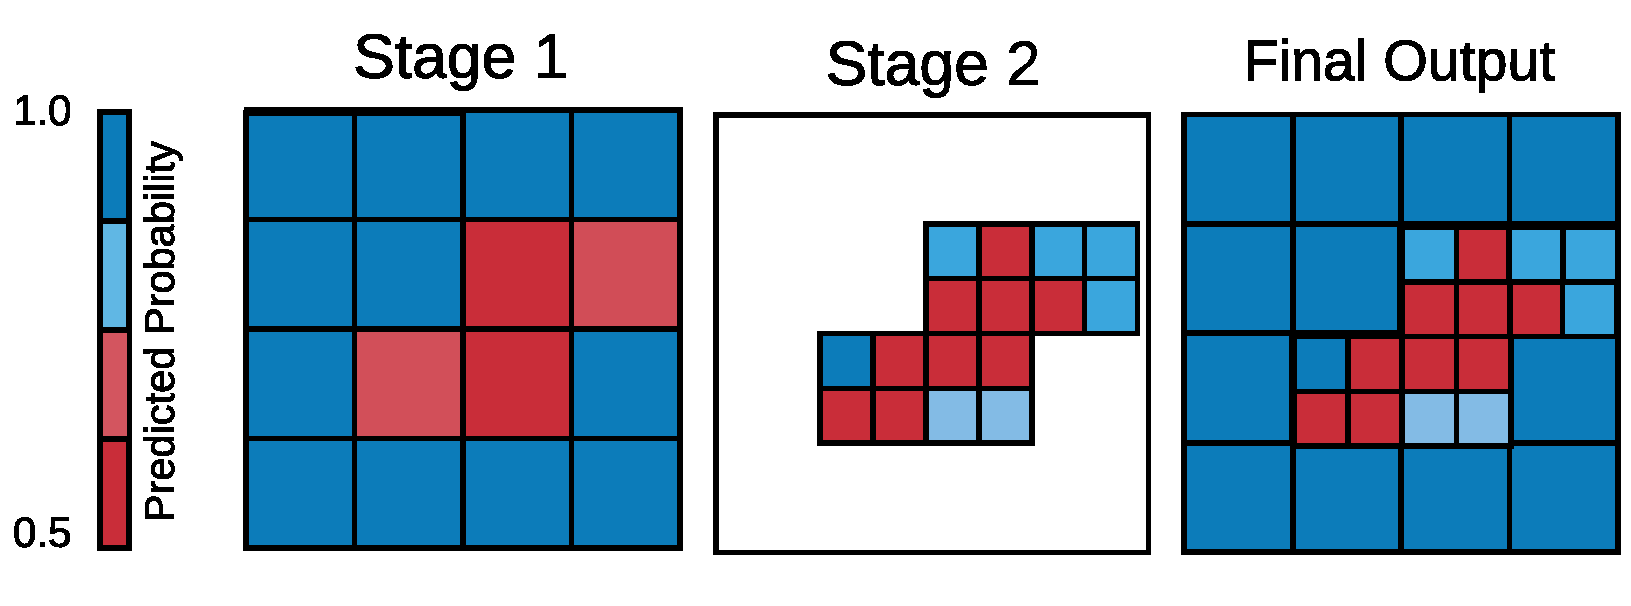
\includegraphics[width=\columnwidth]{images/adaptive-drill-down}
% \caption{Schematic representation of \textit{adaptive drill-down}}
% \label{fig:adaptive-drill-down}
% \end{figure}

\vspace{2mm}
\noindent \textbf{Theoretical Speedups.}
We now define a notion of theoretical speedup for this optimization; this is independent of the theoretical speedup of incremental inference. We first explain the effects of $r_{drill-down}$ and $S_1$. Setting these parameters is an application-specific balancing act. If $r_{drill-down}$ is low, only a small region will need re-inference at the original resolution, which will save a lot of FLOPs. But this may miss some some regions of interest and thus, compromise important explanation details. Similarly, a large $S_1$ also saves a lot of FLOPs by reducing the number of re-inference queries in stage one. But it runs the risk of misidentifying interesting regions, especially when the size of those regions are smaller than the occlusion patch size. We now define the theoretical speedup of adaptive drill-down as the ratio of the number of re-inference queries for regular OBE without this optimization to that with this optimization. We only need the counts, since the occlusion patch dimensions are unaltered, i.e., the cost of a re-inference query is the same with or without this optimization. Given a stride $S$, the number of re-inference queries is $\frac{H_{\mathcal{I}_{img}}}{S} \cdot \frac{W_{\mathcal{I}_{img}}}{S}$. Thus, the theoretical speedup is given by the following equation. Figure~\ref{fig:adaptive_drill_down}(b) illustrates how this ratio varies with $S_1$ and $r_{drill-down}$.

\vspace{-2mm}
\begin{align}
\label{eqn:adaptive-drill-down-eqn}
\texttt{speedup} = \frac{S^2_1}{S^2_2+r_{drill-down} \cdot S^2_1}
\end{align}

\begin{figure}[t]
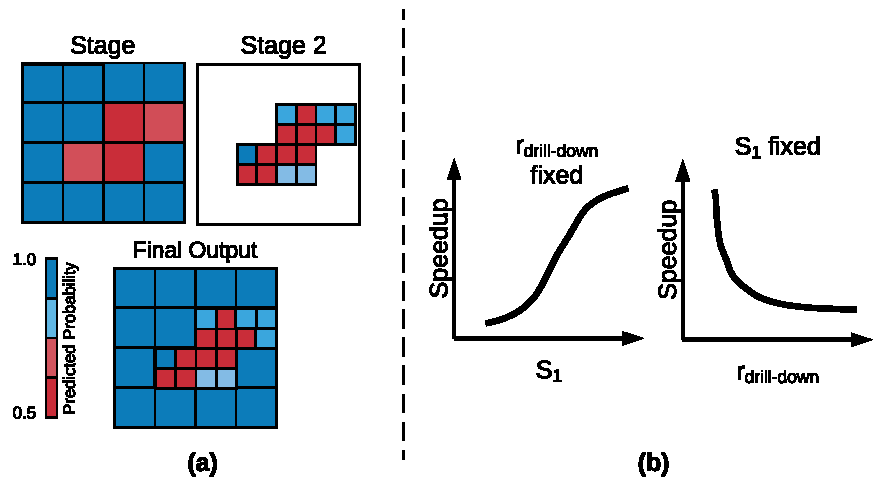
\includegraphics[width=\columnwidth]{images/adaptive_drill_down}
\caption{(a) Schematic illustration of the adaptive drill-down idea. (b) Conceptual depiction of the effects of $S_1$ and $r_{drill-down}$ on the theoretical speedup.. }
\label{fig:adaptive_drill_down}
\vspace{-4mm}
\end{figure}

\subsection{Automated Parameter Tuning}
We now present automated parameter tuning methods for easily configuring our approximate inference optimizations.

\vspace{2mm}
\noindent \textbf{Tuning projective field thresholding.}
As Section 4.1 explained, $\tau$ controls the visual quality of the heat map. There is a spectrum of visual quality degradation: imperceptible changes to major structural changes. But mapping $\tau$ to visual quality directly is likely to be unintuitive for users. Thus, to measure visual quality more intuitively, we adopt a cognitive science-inspired metric called Structural Similarity (SSIM) Index, which is widely used to quantify human-perceptible differences between two images~\cite{wang2004image}. In our case, the two ``images'' are the original and approximate heat maps. SSIM is a number in $[-1,1]$, with $1$ meaning a perfect match. SSIM values in the $[0.90,0.95]$ range are considered almost imperceptible distortions in many practical multimedia applications such as image compression and video encoding~\cite{wang2004image}.

Our tuning process for $\tau$ has an offline ``training'' phase and an online usage phase. The offline phase relies on a set of sample images (default $30$) from the same application domain. We compute SSIM for the approximate and exact heat maps for all sample images for a few $\tau$ values (default $1.0, 0.9, 0.8, \dots, 0.4$). We then learn a second-degree polynomial curve for SSIM as a function of $\tau$ with these data points. Figure~\ref{fig:system_tuning}(a) illustrates this phase and the fit SSIM-$\tau$ curves for 3 different CNNs using sample images from an OCT dataset (Section 5). In the online phase, when OBE is needed on a given image, we expect the user to provide a \textit{target SSIM} for the quality--runtime trade-off they want ($1$ yields the exact heat map). We can then use our learned curve to map this target SSIM to the lowest $\tau$. Figure~\ref{fig:system_tuning}(b) shows the CDFs of differences between the target SSIM ($0.9$) and the actual SSIM yielded when using our auto-tuned $\tau$ on both the training set and a holdout test set (also $30$ images). In $80\%$ of the cases, the actual SSIM was \textit{better} than the user-given target; never once did the actual SSIM go $0.1$ below the target SSIM. This suggests that our auto-tuning method for $\tau$ works, is robust, and applicable to different CNNs.

\vspace{2mm}
\noindent \textbf{Tuning adaptive drill-down.}
As Section~\ref{sec:ada-drill-down} explained, the speedup offered by adaptive drill-down is controlled by two parameters: stage one stride $S_1$ and drill-down fraction $r_{drill-down}$. We expect the user to provide $r_{drill-down}$ (default $0.25$), since it captures the user's intuition about how large or small the region of interest is likely to be in the images in their specific application domain and dataset. We also expect the user to provide a ``target speedup'' ratio (default $3$) for using this optimization to capture their desired quality-runtime trade-off. Higher the user's target speedup, the more we sacrifice the quality of the ``non-interesting regions'' ($1 - r_{drill-down}$ fraction of the heat map). Our automated tuning process sets $S_1$ using these two user-given settings. Unlike the tuning of $\tau$, setting $S_1$ is more direct, since this optimization relies on the number of re-inference queries, not SSIM. Let $\mathit{target}$ denote the target speedup; the original occlusion patch stride is $S_2$. Equation~\ref{eqn:s1} shows how we calculate $S_2$. Since $S_1$ cannot be larger than the image width $W_{img}$ (similarly $H_{img}$) and due to the constraint of $(1-r_{drill\-down} \cdot \texttt{speedup})$ being positive, we also have an upper bound on the possible speedups as per Equation~\ref{eqn:speedup_bound}.

\begin{align}
\label{eqn:s1}
S_1 = &~ \sqrt{\frac{\mathit{target}}{1 - r_{drill-down} \cdot \mathit{target}}} \cdot S_2
\end{align}

\vspace{-2mm}
\begin{align}
\label{eqn:speedup_bound}
\mathit{speedup} < \texttt{min}\Bigg(\frac{W^2_{img}}{S^2_2+r_{drill-down} \cdot W^2_{img}}, \frac{1}{r_{drill-down}}\Bigg)
\end{align}


\begin{figure}[t]
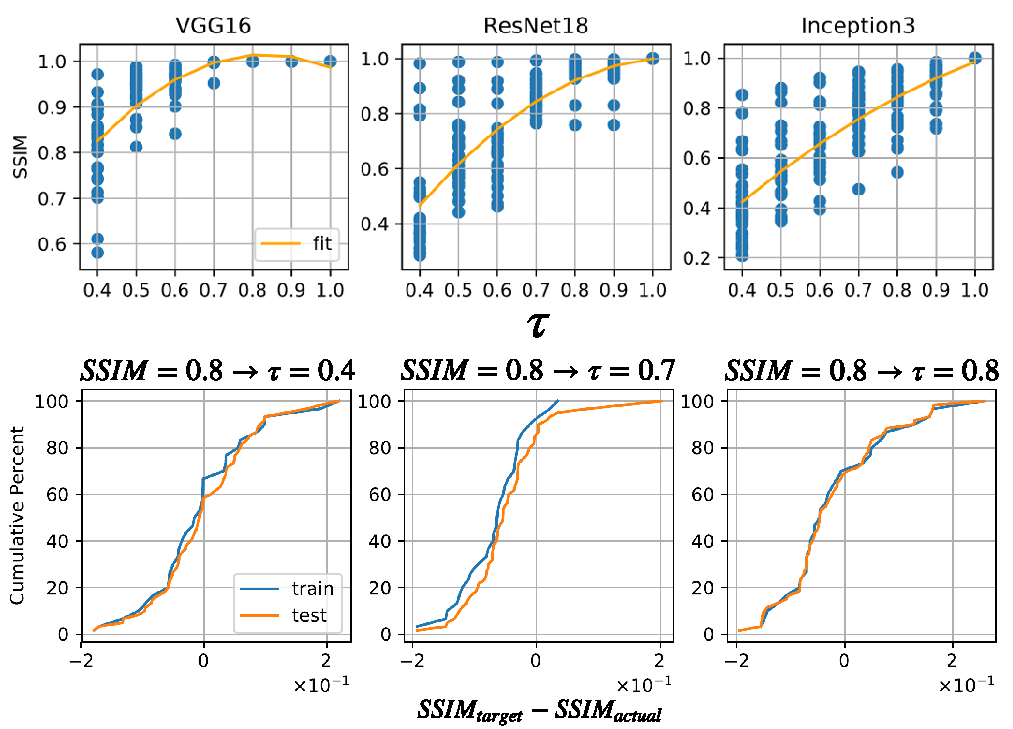
\includegraphics[width=\columnwidth]{images/system_tuning}
\caption{(a) Fitting a second-order curve for SSM against $\tau$ on a sample of the OCT dataset. 
(b) CDFs of deviation of actual SSIM from the target SSIM ($0.9$) with our auto-tuned $\tau$, which turned out to be $0.5$, $0.7$, and $0.9$ for VGG-16, ResNet-18, and Inception-V3, respectively.}
\label{fig:system_tuning}
\vspace{-4mm}
\end{figure}

% \begin{figure}[t]
% 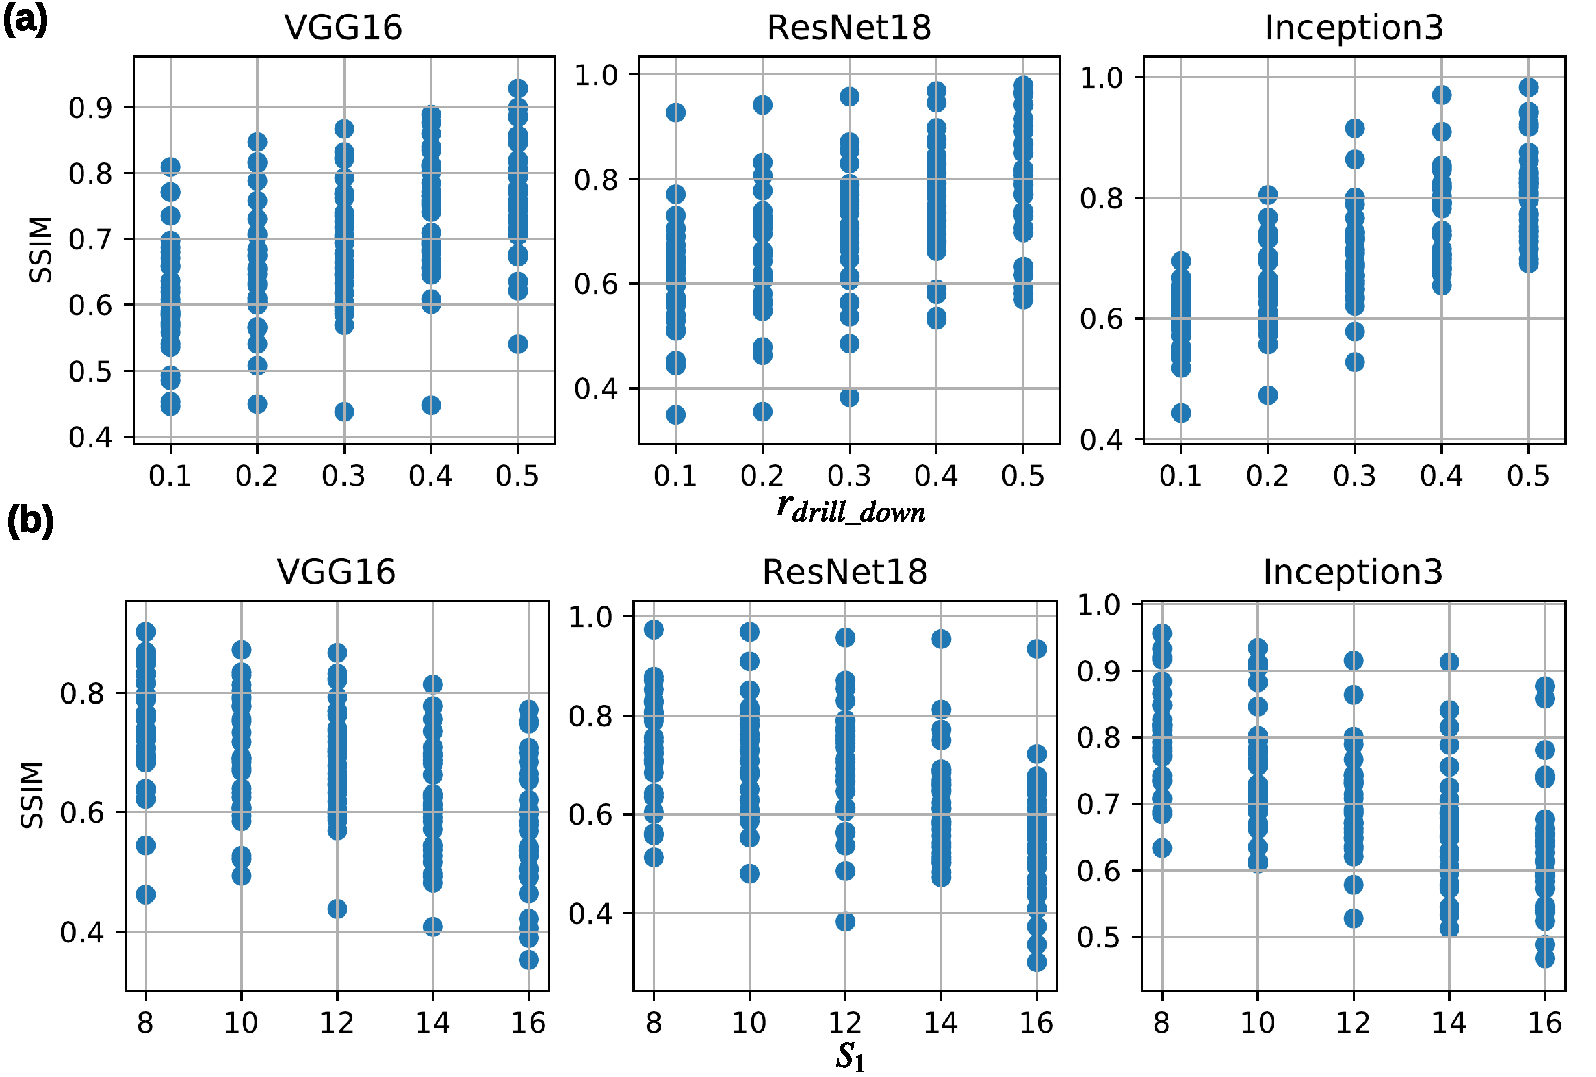
\includegraphics[width=\columnwidth]{images/adaptive_ssim}
% \caption{(a) SSIM variation for changing $r_{drill\_down}$ fixing $\tau=1$, $S_1=12$, and $S_2=4$. (b) SSIM variation for changing $S_1$ fixing $\tau=1.0$, $S_2=4$, and $r_{drill\_down}=0.3$ for a sample $(n=30)$ of OCT dataset.}
% \label{fig:adaptive_ssim}
% \end{figure}

